\chapter{Аналитический раздел}

%\par В этом разделе будет проведён анализ предментой области и обзор существующих решений, обоснована актуальность решаемой продуктом задачи. Также, будет формализована задача, пользовательские сценарии, данные и выбрана модель данных, тип базы данных и тип системы управления базой данных. 

\section{Анализ предметной области}
\par По данным ежегодного отчёта Global Digital 2022, почти 6 из 10 интернет-пользователей трудоспособного возраста (58,4\%) покупают что-то в Интернете каждую неделю~\cite{bib2}. Также, результаты проведённого АКИТ e-commerce анализа показывают, что по сравнению с 2021 годом доля российского рынка интернет-торговли выросла к 2022 году на 1065 миллиардов рублей~\cite{bib3}.

\par В связи с этим, интернет-реклама обрела широкое распространение, как обеспечивающая наиболее эффективное продвижение при помощи механизмов таргетинга~\cite{bib4}. Одним из видов такого продвижения является рекламная рассылка, когда пользователям через каналы обмена сообщениями отправляются письма рекламного характера. Особенно эффективной является персонализированная рекомендательная рассылка, содержание которой формируется на основе предпочтений, так как она позволяет наиболее корректно определять возможные интересы конечного пользователя~\cite{bib5}.

\par Однако, распространение рекламы по сетям электросвязи допускается только при условии предварительного согласия абонента или адресата на её получение~\cite{bib6},~\cite{bib7},~\cite{bib8}. Закон о рекламе не определяет порядка и формы получения согласия, поэтому оно может быть выражено в любой форме~\cite{bib9}. 

\par Подобная рассылка позволяет стимулировать пользователя к возвращению на сайт~\cite{bib4}, подбирать с помощью персонализации актуальные для конкретного пользователя предложения, что увеличивает шанс покупки.

\par Возможна реализация уведомления пользователей о, например, проведении массовых акций, появлении нового ассортимента, предоставлении персональной акции.x

\newpage

\section{Обзор существующих решений}

Для сравнения решений были выбраны критерии:
\begin{enumerate}
	\item Местоположение серверов.
	\item Форма распространения продукта.
	\item Встроенная аналитика.
	\item Ценовая политика.
\end{enumerate}

Было проведено сравнение предложенного решения (SO) с тремя конкурентными: Unisender (U), Mindbox (M), Sendsay (S). По информации, предоставляемой компаниями на сайтах, они являются ведущими в данной сфере~\cite{bib10},~\cite{bib11},~\cite{bib12}. Л.д.~---~личные данные, уст.~---~устанавливаемый, усл.~---~условно.

\begin{table}[H]
	\begin{center}
		\caption{\label{table:cmp} Таблица сравнения существующих решений}
		\begin{tabular}{|c|c|c|c|c|}
			\hline
			{\specialcell{\\Критерий\\}} & \multicolumn{4}{c|}{\specialcell{Решение}}\\ 
			\cline{2-5}
			&{U}&{M}&{S}&{SO}\\ 
		
			\hline
			{\specialcell{Местоположение\\ серверов}} & РФ & РФ & РФ & РФ\\ \hline
			{\specialcell{Форма распр.}} & Облачный & Облачный & Облачный & Уст.\\ \hline
			{\specialcell{Сегментация}} & {\specialcell{По л.д., по \\активности \\с письмами \\и на сайте}} & {\specialcell{По л.д., по \\активности \\на сайте}} & {\specialcell{По л.д., по \\активности \\с письмами}} & {\specialcell{По л.д., по \\активности \\на сайте на \\основе \\аналитики}}\\ \hline
			{\specialcell{Ценовая\\ политика}} & {\specialcell{Усл. беспл.}} & Платно & {\specialcell{Усл. беспл.}} & Бесплатно\\ \hline
			
		\end{tabular}
	\end{center}
\end{table}

Таким образом, предложенное решение, как устанавливаемое, обеспечивает построение независимой от внешних факторов системы и возлагает на пользователя обязанность по выбору защищённой точки хранения, так как происходит работа с персональными данными. Также, данное решение, в отличие от аналогов, является полностью бесплатным и позволяет агрегировать данные о пользовательской активности на сайте, формируя на их основе статистику и более обширную аналитическую сводку, влияющую впоследствии на правила рассылки.

\section{Формализация задачи}
В рамках работы необходимо разработать веб-приложение, обеспечивающее управление рекламной рассылкой на основе данных, получаемых основной торговой площадкой от клиента, при наличии согласия на обработку этих данных. Обрабатываются любые зарегистрированные в системе события, связанные с действиями клиента на сайте. 

Приложение хранит предоставленные личные данные о клиенте и информацию о событиях, связанных с зарегистрированными клиентами. 

Разрабатываемый продукт должен представлять собой приложение модели клиент-сер­вер. Серверная часть приложения отвечает за взаимодействие с хранилищем данных и обработку запросов основной системы, которая подключена к приложению. Клиентская часть представляет собой веб-страницу с пользовательским интерфейсом.

\paragraph{Формализация пользовательских сценариев}\mbox{}

Пользователи системы рассылки~---~таргетологи и администраторы. Клиент основной системы не имеет собственного интерфейса в приложении, но при наличии согласия на обработку персональных данных, запрашиваемого на стороне подключающейся системы, его действия изменяют информацию, хранящуюся в приложении.

На рисунке~\ref{img:use} представлены пользовательские сценарии для реализации.

\newpage

\begin{table}[h!]
  \centering
  \begin{tabular}{p{1\linewidth}}
    \centering
    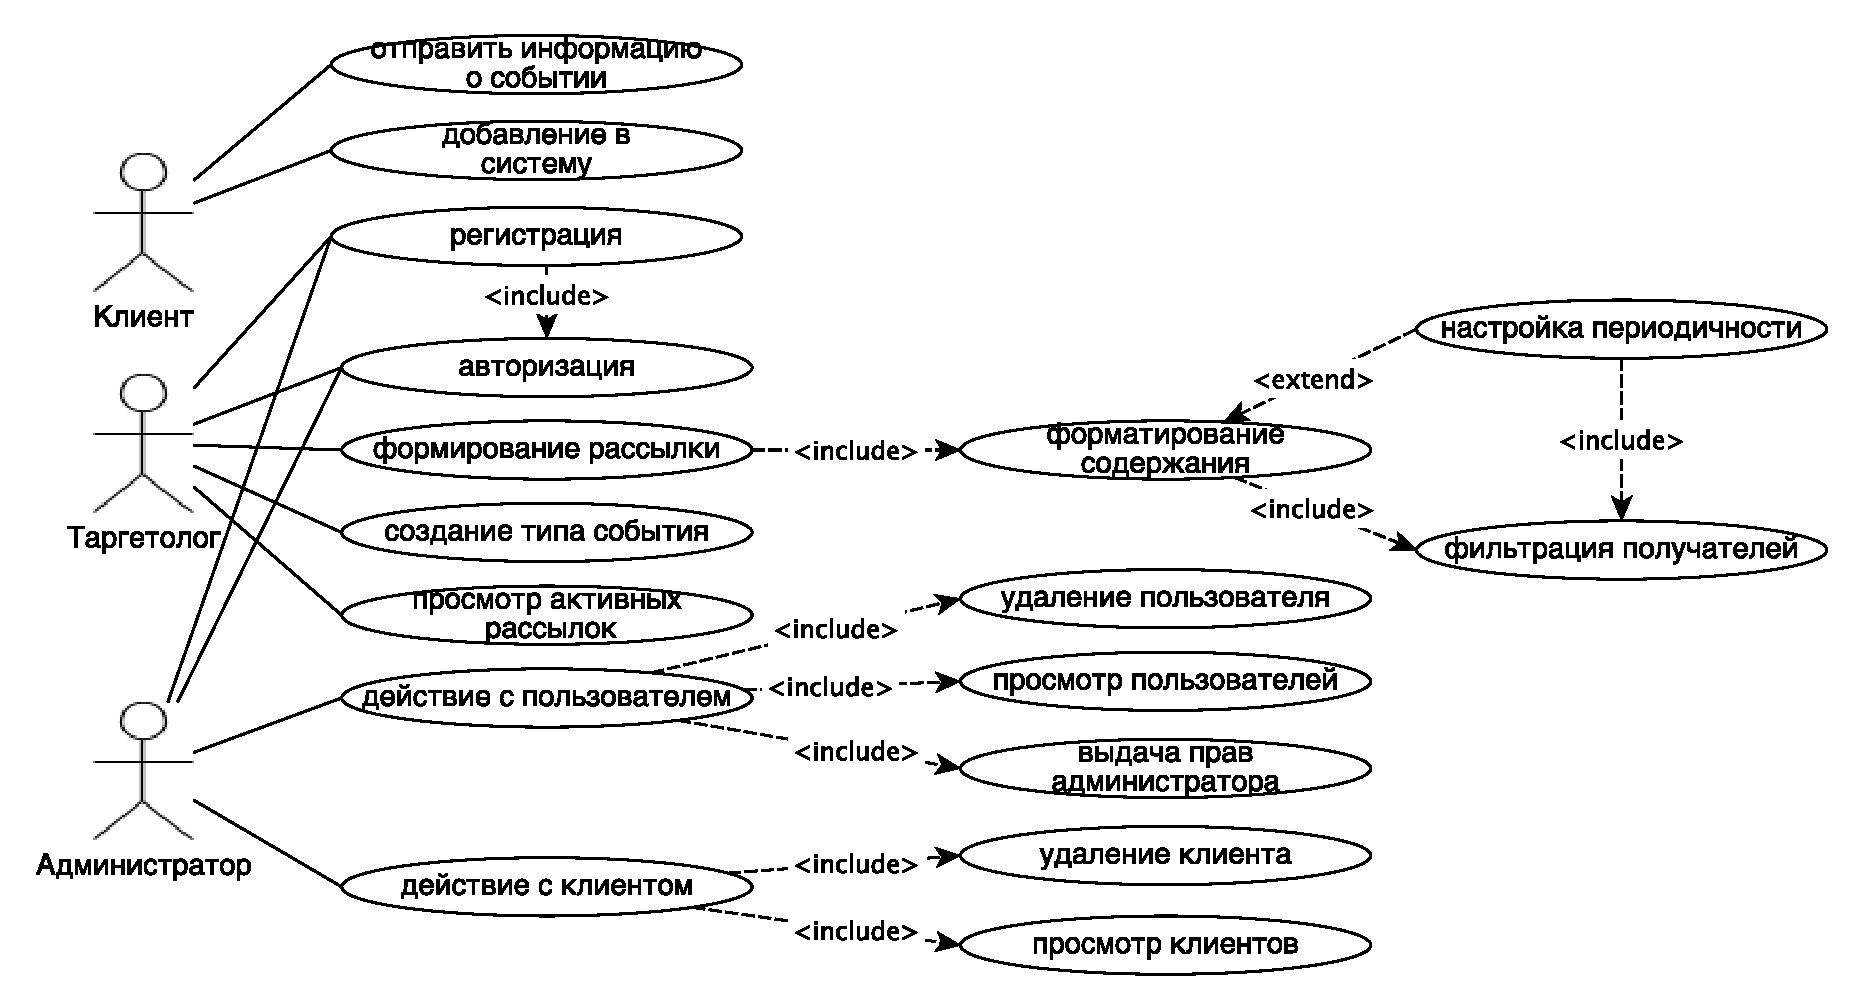
\includegraphics[width=1\linewidth]{./images/use.pdf}
    \captionof{figure}{Пользовательские сценарии}
    \label{img:use}
  \end{tabular}
\end{table}

Таргетологам доступны:
\begin{itemize}
	\item список незавершённых на момент просмотра рассылок;
	\item экран формирования письма: с возможностью форматирования текста письма в HTML и предпросмотра результата, настройки периодичности и  фильтрации;
	\item возможность создания типа события для дальнейшей фильтрации.
\end{itemize}

Администратору доступны функции управления системой верхнего уровня:
\begin{itemize}
	\item просмотр пользователей и клиентов системы;
	\item удаление пользователей и клиентов системы;
	\item выдача прав администратора пользователю.
\end{itemize}

\paragraph{Формализация данных}\mbox{}

Разрабатываемая база данных должна состоять из следующих сущностей:
\begin{enumerate}
	\item Клиент.
	\item Событие.
	\item Пользователь.
	\item Рассылка.
	\item Расписание.
\end{enumerate}

На рисунке~\ref{img:er} представлена ER-диаграмма сущностей в нотации Чена.

\begin{table}[h!]
  \centering
  \begin{tabular}{p{1\linewidth}}
    \centering
    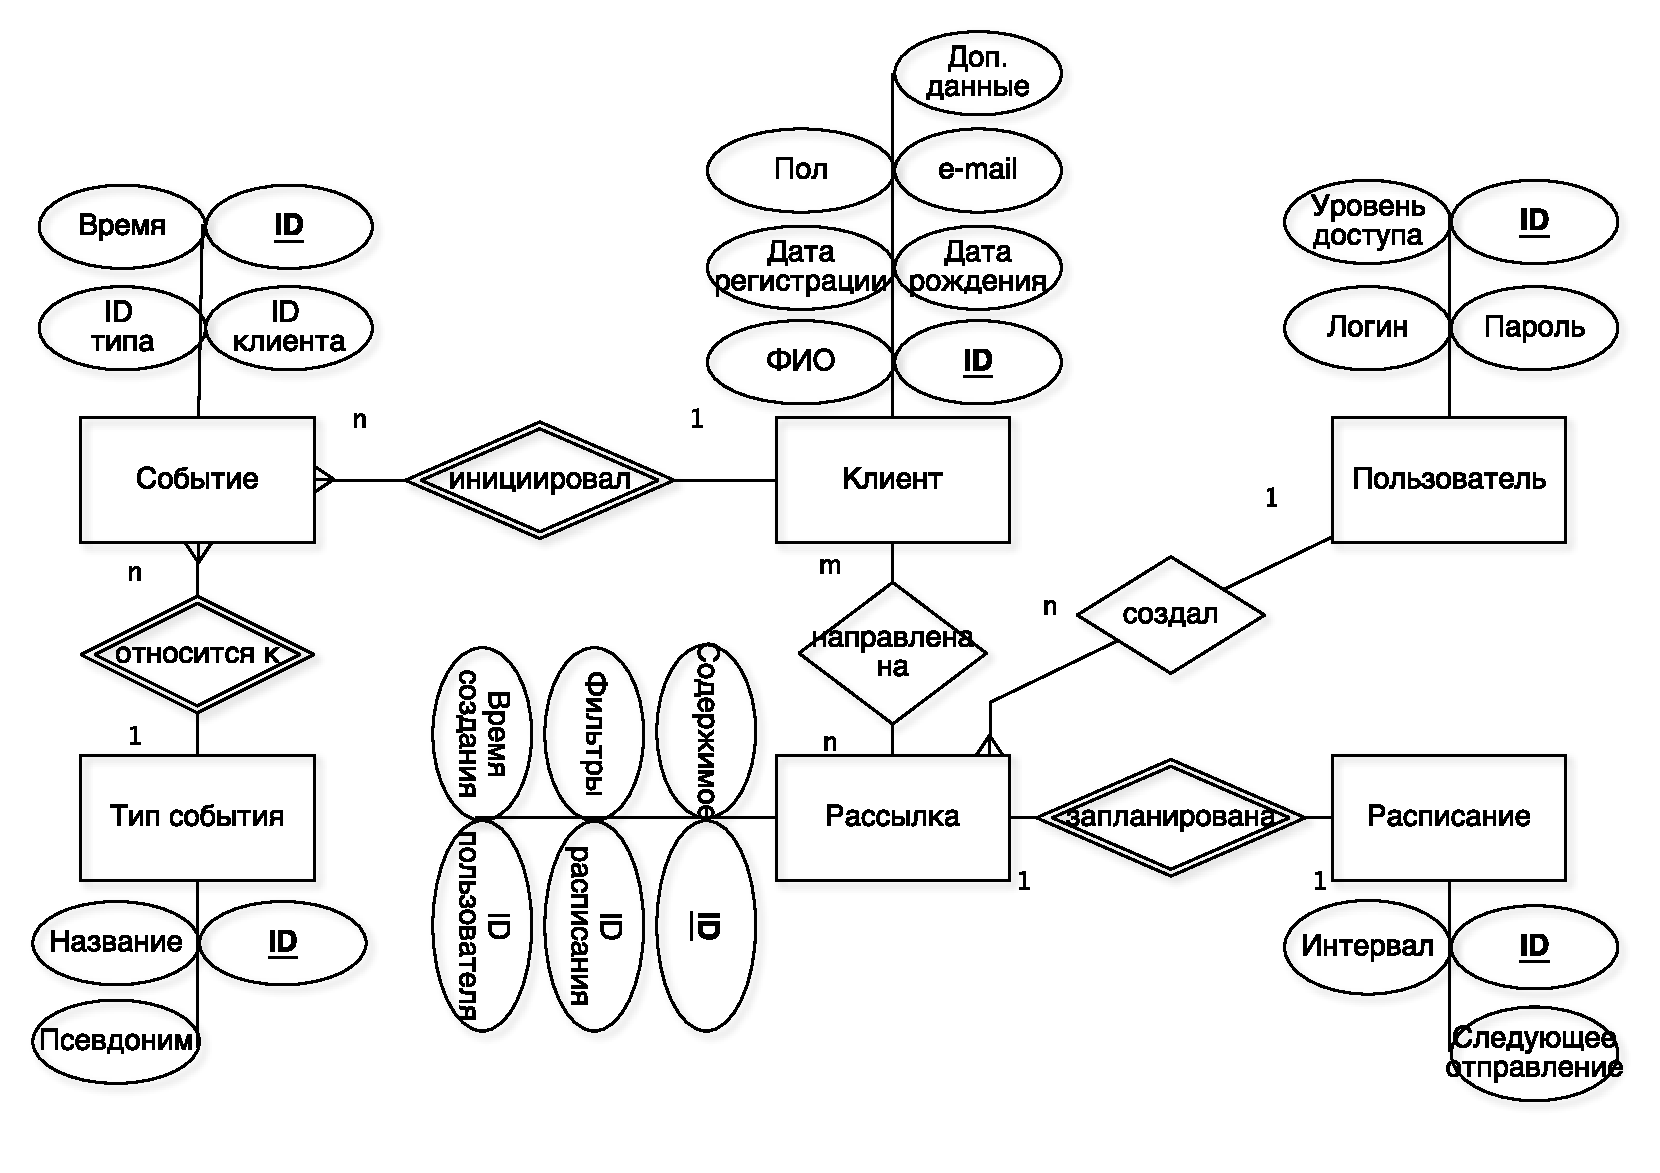
\includegraphics[width=1\linewidth]{./images/er.pdf}
    \captionof{figure}{ER-диаграмма}
    \label{img:er}
  \end{tabular}
\end{table}

\section{Выбор модели данных для базы данных}
Для построения базы данных, как совокупности взаимосвязанных данных некоторой предметной области, необходимо определить базовую модель данных.
Модель данных~---~это абстрактная модель, определяющая совокупность правил создания и использования данных, описывающая способ представления данных, доступ к ним и связи между ними в той или иной области~\cite{bib13}.

\paragraph{Иерархическая модель}\mbox{}

Графически такую модель можно представить в виде графа типа «дерево»~\cite{bib15}. В такой модели имеется одна вершина~---~корень дерева, являющаяся входом в структуру. Каждая вершина, отличная от корня, может иметь только одну исходную вершину и сколько угодно порожденных. В связи с этим является невозможной реализация типа связи «многие ко многим», а так же создание сущности без родительского узла. Направление каждой связи определяется иерархией. Ограничения на тип внутренней структуры отсутствуют, связи задаются адресными указателями, что накладывает обязательство учёта физической организации хранения~\cite{bib19}.

\paragraph{Сетевая модель}\mbox{}

Сетевая модель графически представима в виде графа типа «сеть»~\cite{bib15}. Входом в такую структуру может являться любая вершина. Для одной вершины нет ограничений на количество исходных и ею порождённых. Между парой вершин может существовать более одной связи, поэтому реализация типа связи «многие ко многим» становится возможной. Однако, подобная реализация значительно усложнит схему проектируемой базы данных~\cite{bib20}. Направление и характер связи в сетевых моделях не предопределены, как в иерархической модели, поэтому направление каждой связи должно быть указано. Ограничения на тип внутренней структуры отсутствуют. Связи задаются адресными указателями, что накладывает обязательство учёта физической организации хранения~\cite{bib19}.

\paragraph{Инвертированные списки}\mbox{}

Также, существуют системы, построенные на использовании инвертированных списков~\cite{bib15}. В таких базах данные и информация о связях между элементами данных логически и физически сепарированы. Данные хранятся в файлах сложной структуры, а информация о связях сосредотачивается в отдельных блоках~---~ассоциаторах и сетях связи. В системах, построенных на инвертированных списках, можно реализовывать связь типа «многие ко многим». Отделение ассоциативной информации от хранимых данных позволяет изменять связи, не изменяя при этом сами данные.

\paragraph{Реляционная модель}\mbox{}

Реляционная модель состоит из трех частей: структурной, целостностной и манипуляционной. Структурная часть описывает, из каких объектов состоит реляционная модель. Целостная часть фиксирует базовые требования целостности. Манипуляционная часть описывает способы манипулирования реляционными данными. 

В реляционных базах данные хранятся в форме отношений~---~таблиц, состоящих их записей. Записи имеют линейную структуру~\cite{bib15}. Таблицы могут иметь связи с другими таблицами через внешние ключи, а каждая запись имеет свой уникальный в пределах таблицы идентификатор~---~первичный ключ. Модель поддерживает связи «один к одному» и «один ко многим». Связь «многие ко многим» реализуется с помощью создания связующей сущности. Данная модель характеризуется низкой трудоёмкостью отображения сложных связей между сущностями~\cite{bib19}, наличием строгой регламентации операций над сущностями и правил организации системы хранения, позволяющих избежать дублирования данных~\cite{bib20}.

\section{Выбор базы данных}
Базы данных (БД), по способу хранения, делятся на две группы~---~строковые и колоночные.

\paragraph{Строковые базы данных}\mbox{}

Строковые базы данных~---~это такие базы данных, записи которых в памяти представлены построчно. Для систем, использующих строковые базы, характерно большое количество операций вставки, обновления и удаления данных~\cite{bib18}. Эффективнее будут запросы, обращающихся к отдельным записям. В таких системах мера эффективности~---~количество транзакций в единицу времени.

\paragraph{Колоночные базы данных}\mbox{}

Колоночные базы данных~---~это такие базы данных, записи которых в памяти представляются по столбцам~\cite{bib18}. Колоночные базы данных используется в аналитических системах, где запросы сложнее и включают в себя агрегацию данных. В таких системах мера эффективности~---~время отклика.

\section{Выбор системы управления базами данных}
Система управления базами данных (СУБД)~---~это приложение, обеспечивающее создание, обновление, удаление, хранение и поиск информации в базе данных. По используемой модели данных СУБД делатся на реляционные и нереляционные. Так как выбор уже сделан в пользу реляционной модели, то данные категории рассматриваться не будут. По способу доступа к базе данных СУБД делятся на файл-серверные, клиент-серверные, встраиваемые и прочие. 

\paragraph{Файл-серверные СУБД}\mbox{}

Файл-серверные СУБД~---~это СУБД, у которых файлы данных располагаются локально~\cite{bib14}. На компьютере пользователя запускается копия приложения. По каждому запросу к БД из приложения данные из таблиц БД полностью загружаются на компьютер пользователя, независимо от того, сколько на самом деле данных необходимо для выполнения запроса. Каждый пользователь имеет на своем компьютере локальную копию данных, время от времени обновляемых из реальной БД, расположенной на сетевом сервере. Вся тяжесть выполнения запросов к базе данных и управления целостностью базы данных ложится на приложение пользователя.

\paragraph{Клиент-серверные СУБД}\mbox{}

Клиент-серверная СУБД~---~основанная на технологии «клиент-сервер»~\cite{bib16}. Этот механизм позволяет обмениваться информацией между клиентом и сервером с переносом основной нагрузки на сервер. Клиент только организовывает доступ пользователя к серверу. При направлении запроса к БД клиент получает только искомые записи из-за ненадобности передавать весь массив данных из БД.

\newpage

\paragraph{Встраиваемые СУБД}\mbox{}

Встраиваемые СУБД~---~это СУБД, которые встраиваются в приложения в виде разделяемой программной библиотеки~\cite{bib17}. Встраиваемые СУБД удобно использовать в легковесных приложениях, использующих СУБД для доступа к данным, компьютерных играх, хранящих данные игрового процесса и самой игры, большом количестве приложений, предназначенных для работы на мобильных устройствах. Встраиваемая СУБД локально хранит данные конкретного приложения и не рассчитана на совместное использование. 

\section{Вывод}

В этом разделе был проведён анализ предментой области и обзор существующих решений, обоснована актуальность решаемой продуктом задачи. Также, была формализована задача, пользовательские сценарии и данные. 

Была выбрана реляционная модель данных, как наилучшим образом подходящая для построения системы, подразумевающей нетривиальные связи между сущностями. Отсутствие необходимости изменять структуру данных и возможность исключить дублирование также повлияли на данный выбор.

Для хранения аналитических данных была выбрана колоночная база данных, так как для данного вида информации большую долю запросов будут составлять агрегационные, наиболее оптимально выполнимые в колоночных БД. Для хранения иных данных в работе будет использована строковая БД.

В качестве СУБД была выбрана клиент-серверная, так как данный вариант не накладывает ограничений на объём хранимых данных, и позволяет не манипулировать ненужными в рамках запроса данными.

















 
